\chapter{Implementation}
\label{chapter:implementation}

My experiences during the whole ordeal

\section{Technical decisions}

Picking libraries, choosing languages, determining algorithms, yeah!

\subsection{Generating the routing data}

To create the all-to-all distance matrix necessary for solving the VRP, it is necessary to use a map routing API which computes the distance of the best route between two nodes and estimates the corresponding traveling time. Since there can be hundreds of target locations for the algorithm, it is necessary to group nearby targets into one to limit the number of queries made to the API.

The grouping was performed by picking a random node and assigning its coordinates to other nodes within a 3 kilometre radius. This is then repeated for the remaining untouched nodes until no more merges are possible. While better results could be obtained by picking the merger nodes according to some rules, this simple algorithm is effective enough. The inaccuracy caused by the maximum of 3 kilometre disparity between the real location and the one used for the algorithm should not usually cause big differences in travel time, though with natural formations such as rivers or lakes, this is a possibility.

The number of queries to the map routing API was lowered by 30 - 50 \% by this grouping depending on the test data used. In the number of queries, this provided savings ranging from 1300 to 4000 queries. The more locations involved in the total data, the higher that savings percentage was. This result seems reasonable, as the probability of an additional target being located near an existing one increases as the number of targets increases. The total number of queries made ranged from about 2000 to 4500.

I picked MapQuest\cite{mapquest} to be the routing service provider. They provide 15000 queries per month for free, and that number was high enough for the purpose of this thesis. MapQuest supports getting detailed route information, but for the purpose of this project, only the traveling time value between two locations was used. The routing service provider is easy to replace in the final implementation, as the replacement only requires altering the query made to the service and parsing of the response, so there is no lock-in on a single provider. I tested the quality of MapQuest's routing results by comparing them to the results of other similar services, such as Google maps and Bing maps. The variations between the results was minimal to the point where it was safe to assume that all of them provided good results. 

\subsection{Language requirements}

The most important aspect of choosing which language to use depends on the routing algorithm libraries available for the language. 

Because the algorithm is CPU-intensive, the more low-level languages take precedence over the potentially slower high-level languages. This is not a deciding factor, however, as many of the high-level languages are still sufficiently fast enough for this purpose. Likewise, even if a program written in pure C, for example, might perform better, the increased development time and reduced maintainability are more significant significant issues than a slightly reduced performance of a Java program.

Due to the performance-centric nature of the algorithm, it is important that the language chosen can be profiled to see which parts of the algorithm are the most resource-intensive. Though most modern languages fulfill this requirement, it is worthy of mentioning. 


\subsection{Choosing the libraries to use}

The important criteria for choosing the libraries to use are performance, solution quality and suitability to the parameters specific to this project. Ease of use and the quality of documentation are also signifcant factors.

My main strategy when picking the library to use was to read the API documentation to see if it supported the functionality I need. Since there are so many different variations of the VRP, there are also numerous types of libraries, most of which were specialised for a specific kind of VRP. If a library was aimed for a different purpose it became apparent quickly. Then I examined how well the library has been maintained and how clear the documentation is.

To see if a library was suitable for my requirements, I looked at the API provided by the library and determined if the API supported the functionality I required. If there was no built-in support, I looked how well the library supported writing additional custom constraints to be use in the route generation. I also considered the number and variety of usage examples as one criterion for the decision, as it is a clear indication whether the library supports the various use cases required in the context of this thesis. This method of choosing a library eventually led me to pick Jsprit.
 
This initial choice I made turned out to be a good one and there was little reason to explore other options.



\subsection{Langugage and library decision}
\label{subsection:library and language}

The library I chose for the program was jsprit developed by Stefan Schr�der. TODO: More talk. Cite github repository. https://github.com/graphhopper/jsprit

Jsprit also produces rough visualisations of the best solution it has found, as can be seen in Figure~\ref{fig:librarysolution}.

\begin{figure}[h]
  \begin{center}
    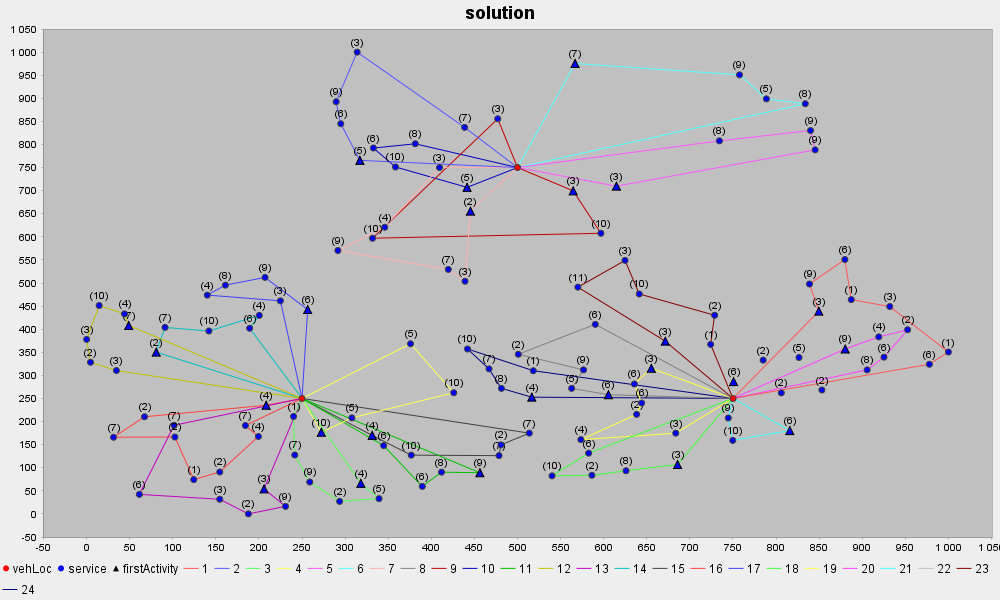
\includegraphics[width=\textwidth]{images/librarysolution.png}
    \caption{An example of the graph output produced by the library}
    \label{fig:librarysolution}
  \end{center}
\end{figure}

Other libraries I researched were (TODO: cite and format properly, explain why they weren't picked)

VRPH: https://sites.google.com/site/vrphlibrary/

Google OR Tools: https://github.com/google/or-tools

Open-VRP: https://github.com/mck-/Open-VRP

VROOM: https://github.com/VROOM-Project/vroom

OptaPlanner: https://www.optaplanner.org

\section{Development of the program}

\subsection{Structure of the program}

To ensure future maintainability, the program was designed to be modular, so if some part of the program needs to changed, the operation will be as easy as possible. The modules of the program are as follows:

\begin{enumerate}  
\item Routing module, transforming address data into a traveling cost matrix. TODO
\item Job resource calculator, abstracting the job resource and man-hour requirements into numbers.
\item The algorithm module, using the traveling cost matrix and job requirements to produce route data.
\item Results visualiser, displaying the results data in a more human-readable form. (not implemented)
\item Results storing module, converting the results into data suitable to be stored in the client company's database. (not implemented) 
\end{enumerate}

 